

\begin{frame}[t]{选题来源}
  在偏微分方程中,对演化方程建立能观测不等式一直是非常重要的课题.考虑薛定谔方程
  \begin{equation}
    i\partial_t u-\Delta u=0,\quad u(0,x)=u_0(x)\in L^2(\Omega),
  \end{equation}
  其中$u_0(x)$是方程的初始函数,上述方程的解函数设为$u(t,x)$.
  
  如果对于某个区域$\omega \subset \Omega$,存在常数$C=C(\omega,T)$使得
  \begin{equation}
    \int_{\omega}|u(T,x)|^2\,\mathrm{d}x\le C \int_0^T\int_{\omega}|u(t,x)|^2\,\mathrm{d}x\mathrm{d}t\label{obs}
  \end{equation}
  成立,我们把该不等式称为给定方程的能观测不等式.
\end{frame}

\begin{frame}[t]{唯一延拓性}
  
  从能观测不等式(\refeq{obs})可以看出:当我们仅仅知道$u(t,x)$在$(0,T)\times \omega$上的信息时,我们可以得到解函数某些解函数整体的性质,在这里就是给出了函数的$L^2$范数上界.
  
  当$u(t,x)$在$[0,T]\times \omega$为零时,可以得到$u=0\in L^2(\Omega)$.这样的性质我们称为唯一延拓性.

  由此可以看出,能观测不等式其实是一种定量唯一延拓性,每一个能观测不等式都能得到一个定性的唯一延拓性.
\end{frame}

\begin{frame}[t]
  近三十年来,人们对于薛定谔方程唯一延拓性和能观测不等式的研究已经有了很多不错的结果:
  \begin{itemize}
    \item G. Lebeau[J. Math. Pures Appl., 1992]证明了边界解析有界区域$\Omega\subset \R^n$上的能观测不等式,观测区域为$(0,T)\times\hat{\omega}$,$\hat{\omega}\subset \partial \Omega$满足几何控制条件(GCC).
    \item K. P. Phung[SIAM J. Control Optim., 2001]证明了有界区域$\Omega$上的齐次薛定谔方程能观测不等式,观测区域为$(0,T)\times \omega$,其中$\omega$是满足几何控制条件的子区域.
    \item Terence Tao在Nonlinear Dispersive Equations一书中,给出了$\R^2$上矩形区域上自由薛定谔方程的能观测不等式,其观测区域为$(0,T)\times \omega$,其中$\omega$可以是任意的非空开子集.
    \item N. Anantharaman和M. L\'{e}autaud[Invent. Math, 2016]给出了二维圆盘上薛定谔方程的能观测不等式,观测区域为$(0,T)\times \omega$,其中$\omega$是非空开子集并且不需要满足几何控制条件.
  \end{itemize}
\end{frame}


\iffalse\begin{frame}[t]
  考虑薛定谔方程 
  \begin{equation}\label{sch}
    i\partial_t u -\Delta u=0,\quad u(0,x)=u_0(x)\in L^2(\R^{n}).
  \end{equation}
 能观测不等式是指下述形式的不等式
 \begin{equation}
   \int_{\Omega}|u(T,x)|^2\,\mathrm{d}x\le C(T,\Omega)\int_{0}^{T}\int_{\omega}|u(t,x)|^2\,\mathrm{d}x\mathrm{d}t,
 \end{equation}
 这里$\omega\subset \Omega$.
 \begin{itemize}
   \item Rosier-Zhang[JDE,2009]证明了全空间情形下有界区域外的可观测性, 即$\omega$ 可取为任意半径的球外.
   \item Jaffard[PM,1990], Komornik-Loreti[2005]证明周期边界条件下任意开集上的可观测性,即$\omega$ 可取为任意开集.
 \end{itemize}
\end{frame}
\fi



\begin{frame}[t]{能观测不等式的新思路}
  前面提到的结果中,观测时间总是一个开区间,即在时间轴上的一个正测度集上稠密.
  
  那么观测时间可以取某种意义上更小的集合吗?

  可以.考虑下述薛定谔方程
  \begin{equation}
    i\partial_t u-\Delta u=0,\quad u(0,x)=u_0(x)\in L^2(\R^n).\label{sch}
  \end{equation}
Gengsheng Wang, Ming Wang, Yubiao Zhang[JEMS, 2019]证明了下述定理
  \begin{alertblock}{薛定谔方程两点时刻能观测不等式} 
    对所有满足方程(\ref{sch})的$u(t,x)$都有
  \begin{equation}\label{obsch}
    \int_{\R^{n}}|u_0(x)|^2\,\mathrm{d}x\le Ce^{\frac{Cr_1 r_2}{t}}\left( \int_{|x|\ge r_1}|u_0(x)|^2\,\mathrm{d}x+\int_{|x|\ge r_2}|u(t,x)|^2 \,\mathrm{d}x \right).
  \end{equation}
  \end{alertblock}
\end{frame}

\begin{frame}[t]{不确定性原理}
  函数$f$ 的傅立叶变换为
  \begin{equation}
    \widehat{f}(\xi):=\int_{\R} f(x)e^{-ix\cdot \xi}\,\mathrm{d}\xi.
  \end{equation}
  调和分析中的不确定性原理告诉我们:如果一个函数及其傅立叶变换在无穷远处等于$0$,则这个函数恒为$0$.


  Logvinenko-Sereda[Teor. Funkc. Funkc. Anal., 1974]证明了
 \begin{equation}\label{unc}
   \int_{\R^{n}}|f(x)|^2\,\mathrm{d}x\le C e^{Cr_1r_2}\left( \int_{|x|\ge r_1}|f(x)|^2\,\mathrm{d}x+\int_{|x|\ge r_2}|\widehat{f}(\xi)|^2\,\mathrm{d}\xi \right).
 \end{equation}
 不确定性原理有许多不同控制区域的版本,而之前提到的定理完整版其实就是建立了不确定性原理和两点能观测不等式的等价关系.
\end{frame}

\begin{frame}[t]{两点能观测不等式的特点}
  \begin{itemize}
    \item 该不等式一改之前时间上必须是开区间的限制,把一段时间改进到了两点时刻.在此之前,全空间情形下的结果只有在一段时间上有界区域外的能观测不等式,该结果由Rosier-Zhang[JDE, 2009]证明.
    \item 建立了能观测不等式和不确定性原理的等价性.
    \item 常数关于$r_1,r_2$的依赖关系是最优估计,相应的两点时刻也是最优.
  \end{itemize}
%  在此结果出现之前,绝大多数关于薛定谔方程的能观测不等式都是建立在某一时间区间上的,而(\ref{obsch})中只取两个时刻的球外进行观测便能控制住整体.所以这是一个非常新颖的结果.
\end{frame}


\begin{frame}[t]{KdV方程的定性唯一延拓性}
  考虑下述线性 Korteweg-de Vries (KdV) 方程
  \begin{equation}\label{kdv}
    \partial_t u +\partial_x^3u=0,\quad u(0,x)=u_0(x)\in L^2(\R).
  \end{equation}
一个自然而然的问题是,KdV方程是不是也有类似的两点能观测不等式?
\end{frame}

\begin{frame}[t]
  KdV方程在这方面的结果和薛定谔方程类似,有许多定性的唯一延拓性:
  \begin{itemize}
    \item {}[B.Y. Zhang,SIAM J. Math. Anal., 1992] 若$u$在 $(-\infty,c)\times {t_0,t_1}$上等于零,则$u\equiv 0$.
    \item {}[J. Bourgain, IMRN, 1997] 若$u$在球外的一段时间等于零,则 $u\equiv 0$,这对非线性情形也成立.
    \item {}[Kenig et.al., JFA, 2007; Bull. AMS, 2012] 当$u$在 $t_0,t_1$处指数衰减,则$u\equiv 0$.
  \end{itemize}
\end{frame}
\begin{frame}[t]{KdV方程两点能观测不等式}
  Ze Li, Ming Wang[SIAM J. Math. Anal., to appear]证明了下述两点能观测不等式:
  \begin{alertblock}{KdV方程两点时刻能观测不等式} 
    对所有满足方程(\ref{kdv})的$u(t,x)$都有
  \begin{equation}
    \int_{\R^{n}}|u_0(x)|^2\,\mathrm{d}x\le Ce^{Ct ^{-\frac{4}{3}}\left(r_1^4+r_2^4\right)}\left( \int_{B_{r_1}^c}|u_0(x)|^2\,\mathrm{d}x+\int_{B_{r_2}^c}|u(t,x)|^2 \,\mathrm{d}x \right).\label{kdv-obs-old}
  \end{equation}
\end{alertblock}
  该不等式与之前的两点能观测不等式一样,具有相同的形式,但是这个结果无法说明对所有的可测集外都成立,只能对有界可测集区域外成立.
  
  我们的研究方向就是突破$B_{r_1}$和$B_{r_2}$这种有界的限制,甚至突破有限测度的限制. 
\end{frame}
\begin{frame}[t]{主要结果I}
  \begin{alertblock}{KdV上两点时刻可测集外能观测不等式}
    若$|S|,|\Sigma|<\infty$,对于任意的$t>0$,存在常数 $C=C(t,S,\Sigma)>0$使得
    \[ 
    \partial_t u +\partial_x^3u=0,\quad u(0,x)=u_0(x)\in L^2(\R).
    \] 
    所有解$u(t,x)$ 满足
  \begin{equation}\label{obkdv}
    \int_{\R}|u_0(x)|^2\,\mathrm{d}x\le C \left( \int_{\R\setminus S}|u_0(x)|^2\,\mathrm{d}x + \int_{\R\setminus \Sigma} |u(t,x)|^2\,\mathrm{d}x  \right). 
  \end{equation}
  \end{alertblock}
  对比上一个KdV能观测不等式的结果,它们的区别是:
  \begin{alertblock}{}
    集合$|S|,|\Sigma|$比上一情形更广泛.后者必须满足$S\subset B_{r_1}(0),\Sigma\subset B_{r_2}(0),r_1,r_2>0$.
  \end{alertblock}
  例如,对于集合$S=\Sigma=\bigcup_{n=1}^\infty \left(n,n+\frac{1}{n^2}\right)$,显然它们都是有限可测集,但是它
\end{frame}

\begin{frame}[t]
  们是无界的,即不包含在任何有界区域内.所以对于无界有限测度集合,Ze Li和Ming Wang证明的(\ref{kdv-obs-old})就无能为力,而新的KdV能观测不等式则成立.代价是失去了精确的常数估计.
\end{frame}


\iffalse
\begin{frame}[t]
  Consider the following linear Korteweg-de Vries (KdV) equation
  \begin{equation}\label{3}
    \partial_t u +\partial_x^3u=0,\quad u(0,x)=u_0(x)\in L^2(\R).
  \end{equation}
  Our aim is to prove the observability inequality at two points in time as (\ref{obsch}) for (\ref{3}),

%  The solution of (\ref{3}) is expressed by 
%  \begin{equation}\label{4}
%    u(t,x)=\int_{-\infty}^{\infty}E(t,x-y)u_0(y)\,\mathrm{d}y,
%  \end{equation}
%  where $K(\cdot ,\cdot )$ is given by
%  \begin{equation}
%    E(t,x)=\begin{cases}
%      \frac{1}{3t ^{\frac{1}{3}}}\mathrm{Ai}\left( \frac{x}{\left( 3t \right) ^{\frac{1}{3}}} \right), & t>0 \\
%      \delta(x), & t=0.
%    \end{cases}
%  \end{equation}
%  Here, $\mathrm{Ai}(w)$ is the Airy function defined via 
%  \begin{equation}
%    \mathrm{Ai}(w)=\frac{1}{2\pi}\int_{-\infty}^{\infty}e^{iwz+\frac{1}{3}z^3}\, \mathrm{d}z.
%  \end{equation}
  i.e.,
  \begin{equation}\label{7}
    \int_{\R}|u_0(x)|^2\,\mathrm{d}x\le C \left( \int_{\R\setminus S}|u_0(x)|^2\,\mathrm{d}x + \int_{\R\setminus \Sigma} |u(t,x)|\,\mathrm{d}x  \right), 
  \end{equation}
  where $C$ is a constant depending on $t$ and finite sets $S$ and $\Sigma$. 
\end{frame}
\fi

\begin{frame}[t]{主要难点}
  对于薛定谔方程的解$u(t,x)$,可以写成
  \[
    u(x,t)=\int_{\R^{n}}\frac{e^{i|x-y|^2 /4t} }{(4\pi it)^{n /2}}u_0(y)\,\mathrm{d}y.
  \] 
  由此可以推出以下关系式
  \begin{equation}\label{rel}
    (2it)^{\frac{n}{2}}e^{-i|x|^2 /4t}u(x,t)=\widehat{e^{i|\cdot |^2 /4t}u_0}(x /2t), \text{ for all }t>0.
  \end{equation}
  该式说明$t$ 时刻的解在去掉一个模为1的因子外,可以看成是初值的傅立叶变换.因此可以借助于不确定性原理的思想来得到相应的能观测不等式.

如果将KdV方程的解写成上述的积分表示,积分核没有显式表示,因此失去了与不确定性原理的联系.

为了绕过这一障碍,Ze Li, Ming Wang对将观测区域进一步限制为球外,这一限制让它们得以运用解析工具构造出相应的能观测不等式.

\end{frame}
\begin{frame}[t]{主要难点}
  在我们的主要结果中I中,取消了有界性这一限制,这使得我们不得不放弃运用解析性质的思路,另辟蹊径.我们最终选择了更加一般化的算子方法,从而去除了有界的限制.

  但是另一方面,我们也牺牲了精确的常数依赖关系.
\end{frame}

\begin{frame}[t]{证明思路}

\begin{enumerate}
  \item [(1)] 设$S,\Sigma$为给定的有限测度集合,构造算子
    \begin{equation}
      Tf:=\chi_{S} S(t)\chi_{\Sigma}f ,\quad f\in L^2(\R). 
    \end{equation}
    其中$\chi_S,\chi_\Sigma$为示性函数,$S(t)$定义为
   \begin{equation}
     u(t,x)=S(t)u_0(x).
   \end{equation}
\item [(2)] 证明$T$ 是紧算子.利用$S(t)$的积分核逐点估计尝试证明 $T$是Hilbert-Schimdt算子,从而是紧算子.
\item [(3)] 证明$\|T\|<1$.容易证明$\|T\|\le 1$,再由反证法及(2)证明其范数不可能等于$1$.
\item [(4)]  证明两点能观测不等式,由(3)以及KdV的守恒律得到.
\end{enumerate} 
\end{frame}
\iffalse
\begin{frame}[t]
  The strategy to prove (\ref{7}) is to construct the operator
  \begin{equation}\label{8}
    Tf := \chi_{S}S(-t)\left( \chi_{\Sigma}S(t)f \right).  
  \end{equation}
  and claim that $T$ is a compact operator and $\|T\|<1$.

 \begin{equation}
   Tf(x)=\int \chi_{S}(x)\left( \int E(-t,x-w)\chi_\Sigma(w) E(t,w-y)\,\mathrm{d}w \right) f(y)\,\mathrm{d}y.
 \end{equation}
 Define $K(x,y)=\chi_S(x)\int E(-t,x-w)\chi_{\Sigma}(w)E(t,w-y)\,\mathrm{d}w $. Then 
\begin{equation}
  Tf(x)= \int K(x,y)f(y)\,\mathrm{d}y.
\end{equation}

\end{frame}
\fi
%\begin{frame}[t]
%  By the conservation law, we have $\|S(t)\|_{L^2}=1$, Hence $\|T\|\le 1$. Hilbert-Schmidt norm of $T$ is finite. It follows that $T$ is a compact operator.
%\end{frame}
\begin{frame}[t]{集合密度}
  接下来我们想在原有的方法基础上,突破测度有限的限制.

  我们需要引入下述定义
  \begin{block}{$|x|^{-\alpha}$密度集}
    一个可测集$A$称为具有$|x|^{-\alpha}$密度,如果其满足:对于一个给定的$\alpha>0$,有下式成立
    \begin{equation}
      \varlimsup_{x\to \infty}|A\cap [x,x+1]|\lesssim|x|^{-\alpha}.
    \end{equation}
  \end{block}
\end{frame}

\begin{frame}[t]{主要结果II}
  有了集合密度的定义,我们就可以用它来表述我们第二个结果:
  \begin{alertblock}{测度可能无限的能观测不等式}
    设$S$和$\Sigma$均为密度$\alpha>\frac{5}{6}$,并且$S,\Sigma \subset (c,\infty)$或者$S,\Sigma\subset (-\infty,c)$,其中$c\in \R$为一个常数.则对任意的$t>0$,存在常数$C=C(t,\alpha)>0$使得能观测不等式(\ref{obkdv})仍然成立.
  \end{alertblock}
  该结果的证明需要对之前证明中的第三步进行修改,需要结合B. Y. Zhang[SIAM J. Math. Anal., 1992]在半轴上的唯一延拓性结论.
\end{frame}

\begin{frame}[t]{举例与讨论}
  为了满足定理的密度条件,我们可以设集合
  \begin{equation}
    S=\Sigma=\bigcup_{n=1}^{\infty}[n,n+\frac{1}{n^{\frac{5.1}{6}}}].
  \end{equation}
  显然$S$和$\Sigma$都满足定理的条件,并且测度无限,所以这是和之前所有能观测不等式都不一样的新结果.

  实际上,定理中对于密度的限制经过仔细计算后,可以放宽为
  \begin{equation}
    \begin{cases}
      \alpha+\beta>\frac{5}{3}, &\\
      \alpha+3\beta>3, &\\
      3\alpha+\beta>3,&\\
      \alpha,\beta>\frac{1}{2}.&

    \end{cases}
  \end{equation}
  其中$\alpha$和$\beta$分别是$S$和$\Sigma$的密度.
\end{frame}
\begin{frame}[t]
  上述区域可以用图像表示为
  \begin{figure}[ht]
    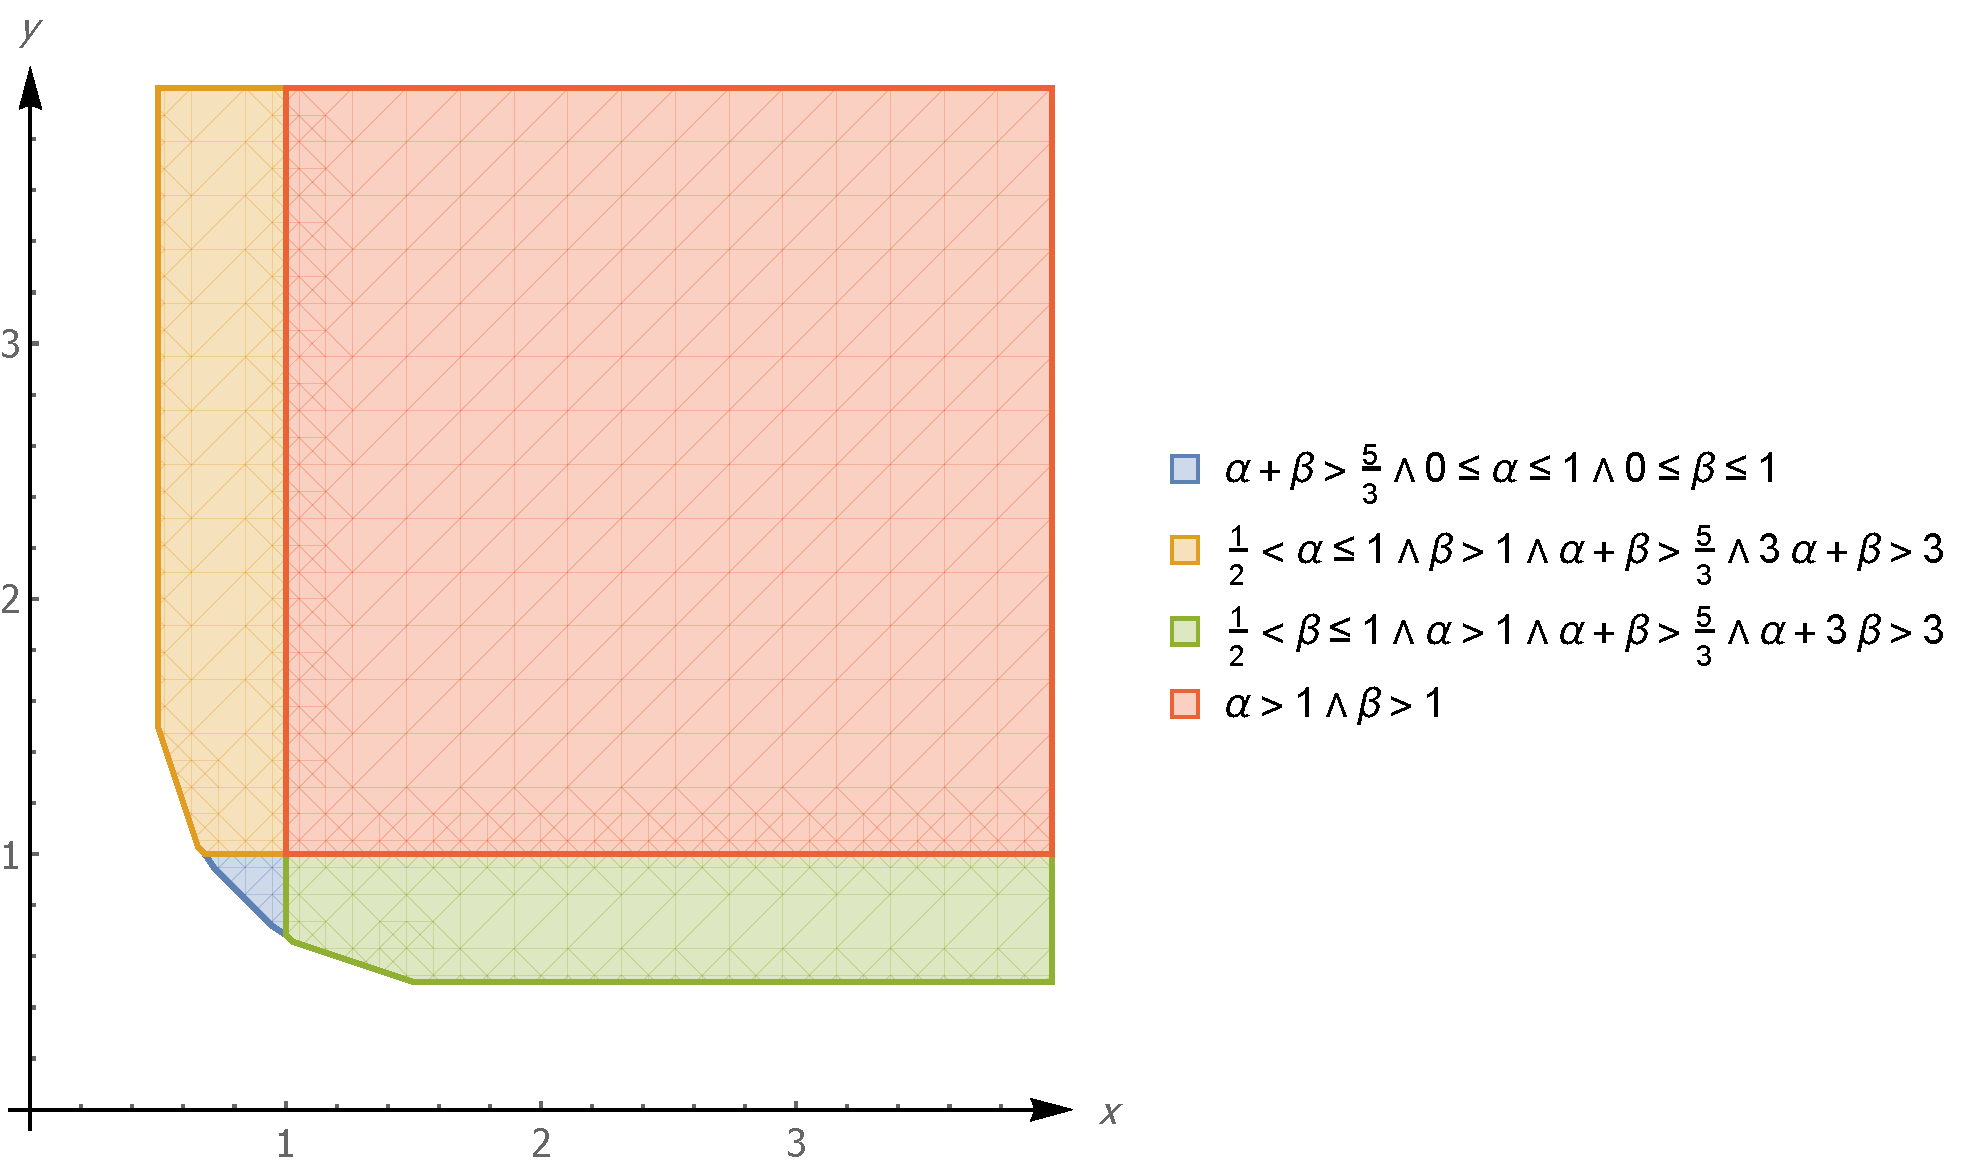
\includegraphics[width=8cm]{range.pdf}
    \centering
    \caption{能观测不等式成立区域,蓝色为可构造无限测度区域}
    \label{fig1}
    \end{figure}
\end{frame}
\begin{frame}[t]{方法的推广}
  我们使用的算子方法并不仅仅局限于各种演化方程的演化算子$S(t)$,只要是满足条件的算子均可以建立类似的不等式.

  例如,对于著名地Hilbert算子
  \begin{equation}
    Hf(x)\equiv \mathrm{p.v.}\frac{1}{\pi}\int_{\R}\frac{f(x-t)}{t}\,\mathrm{d} t,
  \end{equation}
  集合其在任意有限测度上的反局部性,利用上述的证明方法便可得到不等式
  \begin{equation}
    \int_{\R}|f|^2\,\mathrm{d} x\le C\left(\int_{A^c} |f|^2\mathrm{d} x+\int_{B^c}|Hf|^2\,\mathrm{d} x\right).
  \end{equation}
\end{frame}

\begin{frame}[t]{进一步地思考}
  我们已经对于可测集和部分无限测度的集合建立了能观测不等式,但是从我们的方法上看,我们给的条件并不够本质.也就是说,应该可以把条件放宽到更一般的情形,这就是我们下一步努力的目标.
  \begin{center}
   \Huge\bf 谢谢!
  \end{center}
\end{frame}
